\documentclass[tikz, margin=3.14mm]{standalone}

\usepackage{tikz}

\usetikzlibrary{decorations, calc, arrows, arrows.meta, positioning}

\begin{document}
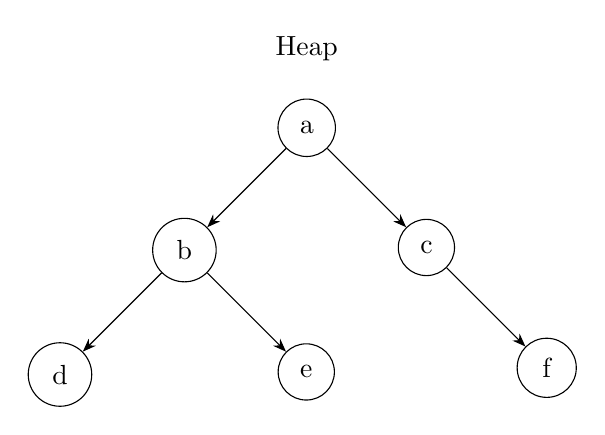
\begin{tikzpicture}[
    >=Stealth,
    heap/.style={circle, draw, inner sep=5pt}
]

% Nodes ------------------------------------------------------

\node (title) at (0,1) {Heap};

\node[heap] (n1) {a};
\node[heap, below left=of n1] (n2) {b};
\node[heap, below right=of n1] (n3) {c};
\node[heap, below left=of n2] (n4) {d};
\node[heap, below right=of n2] (n5) {e};
\node[heap, below right=of n3] (n6) {f};

% Arrows ---------------------------------------------------

\draw [->] (n1) -- (n2);
\draw [->] (n1) -- (n3);
\draw [->] (n2) -- (n4);
\draw [->] (n2) -- (n5);
\draw [->] (n3) -- (n6);
    
\end{tikzpicture}
\end{document}